% Options for packages loaded elsewhere
\PassOptionsToPackage{unicode}{hyperref}
\PassOptionsToPackage{hyphens}{url}
%
\documentclass[
  man,floatsintext]{apa6}
\usepackage{amsmath,amssymb}
\usepackage{iftex}
\ifPDFTeX
  \usepackage[T1]{fontenc}
  \usepackage[utf8]{inputenc}
  \usepackage{textcomp} % provide euro and other symbols
\else % if luatex or xetex
  \usepackage{unicode-math} % this also loads fontspec
  \defaultfontfeatures{Scale=MatchLowercase}
  \defaultfontfeatures[\rmfamily]{Ligatures=TeX,Scale=1}
\fi
\usepackage{lmodern}
\ifPDFTeX\else
  % xetex/luatex font selection
\fi
% Use upquote if available, for straight quotes in verbatim environments
\IfFileExists{upquote.sty}{\usepackage{upquote}}{}
\IfFileExists{microtype.sty}{% use microtype if available
  \usepackage[]{microtype}
  \UseMicrotypeSet[protrusion]{basicmath} % disable protrusion for tt fonts
}{}
\makeatletter
\@ifundefined{KOMAClassName}{% if non-KOMA class
  \IfFileExists{parskip.sty}{%
    \usepackage{parskip}
  }{% else
    \setlength{\parindent}{0pt}
    \setlength{\parskip}{6pt plus 2pt minus 1pt}}
}{% if KOMA class
  \KOMAoptions{parskip=half}}
\makeatother
\usepackage{xcolor}
\usepackage{graphicx}
\makeatletter
\def\maxwidth{\ifdim\Gin@nat@width>\linewidth\linewidth\else\Gin@nat@width\fi}
\def\maxheight{\ifdim\Gin@nat@height>\textheight\textheight\else\Gin@nat@height\fi}
\makeatother
% Scale images if necessary, so that they will not overflow the page
% margins by default, and it is still possible to overwrite the defaults
% using explicit options in \includegraphics[width, height, ...]{}
\setkeys{Gin}{width=\maxwidth,height=\maxheight,keepaspectratio}
% Set default figure placement to htbp
\makeatletter
\def\fps@figure{htbp}
\makeatother
\setlength{\emergencystretch}{3em} % prevent overfull lines
\providecommand{\tightlist}{%
  \setlength{\itemsep}{0pt}\setlength{\parskip}{0pt}}
\setcounter{secnumdepth}{-\maxdimen} % remove section numbering
% Make \paragraph and \subparagraph free-standing
\ifx\paragraph\undefined\else
  \let\oldparagraph\paragraph
  \renewcommand{\paragraph}[1]{\oldparagraph{#1}\mbox{}}
\fi
\ifx\subparagraph\undefined\else
  \let\oldsubparagraph\subparagraph
  \renewcommand{\subparagraph}[1]{\oldsubparagraph{#1}\mbox{}}
\fi
\newlength{\cslhangindent}
\setlength{\cslhangindent}{1.5em}
\newlength{\csllabelwidth}
\setlength{\csllabelwidth}{3em}
\newlength{\cslentryspacingunit} % times entry-spacing
\setlength{\cslentryspacingunit}{\parskip}
\newenvironment{CSLReferences}[2] % #1 hanging-ident, #2 entry spacing
 {% don't indent paragraphs
  \setlength{\parindent}{0pt}
  % turn on hanging indent if param 1 is 1
  \ifodd #1
  \let\oldpar\par
  \def\par{\hangindent=\cslhangindent\oldpar}
  \fi
  % set entry spacing
  \setlength{\parskip}{#2\cslentryspacingunit}
 }%
 {}
\usepackage{calc}
\newcommand{\CSLBlock}[1]{#1\hfill\break}
\newcommand{\CSLLeftMargin}[1]{\parbox[t]{\csllabelwidth}{#1}}
\newcommand{\CSLRightInline}[1]{\parbox[t]{\linewidth - \csllabelwidth}{#1}\break}
\newcommand{\CSLIndent}[1]{\hspace{\cslhangindent}#1}
\ifLuaTeX
\usepackage[bidi=basic]{babel}
\else
\usepackage[bidi=default]{babel}
\fi
\babelprovide[main,import]{english}
% get rid of language-specific shorthands (see #6817):
\let\LanguageShortHands\languageshorthands
\def\languageshorthands#1{}
% Manuscript styling
\usepackage{upgreek}
\captionsetup{font=singlespacing,justification=justified}

% Table formatting
\usepackage{longtable}
\usepackage{lscape}
% \usepackage[counterclockwise]{rotating}   % Landscape page setup for large tables
\usepackage{multirow}		% Table styling
\usepackage{tabularx}		% Control Column width
\usepackage[flushleft]{threeparttable}	% Allows for three part tables with a specified notes section
\usepackage{threeparttablex}            % Lets threeparttable work with longtable

% Create new environments so endfloat can handle them
% \newenvironment{ltable}
%   {\begin{landscape}\centering\begin{threeparttable}}
%   {\end{threeparttable}\end{landscape}}
\newenvironment{lltable}{\begin{landscape}\centering\begin{ThreePartTable}}{\end{ThreePartTable}\end{landscape}}

% Enables adjusting longtable caption width to table width
% Solution found at http://golatex.de/longtable-mit-caption-so-breit-wie-die-tabelle-t15767.html
\makeatletter
\newcommand\LastLTentrywidth{1em}
\newlength\longtablewidth
\setlength{\longtablewidth}{1in}
\newcommand{\getlongtablewidth}{\begingroup \ifcsname LT@\roman{LT@tables}\endcsname \global\longtablewidth=0pt \renewcommand{\LT@entry}[2]{\global\advance\longtablewidth by ##2\relax\gdef\LastLTentrywidth{##2}}\@nameuse{LT@\roman{LT@tables}} \fi \endgroup}

% \setlength{\parindent}{0.5in}
% \setlength{\parskip}{0pt plus 0pt minus 0pt}

% Overwrite redefinition of paragraph and subparagraph by the default LaTeX template
% See https://github.com/crsh/papaja/issues/292
\makeatletter
\renewcommand{\paragraph}{\@startsection{paragraph}{4}{\parindent}%
  {0\baselineskip \@plus 0.2ex \@minus 0.2ex}%
  {-1em}%
  {\normalfont\normalsize\bfseries\itshape\typesectitle}}

\renewcommand{\subparagraph}[1]{\@startsection{subparagraph}{5}{1em}%
  {0\baselineskip \@plus 0.2ex \@minus 0.2ex}%
  {-\z@\relax}%
  {\normalfont\normalsize\itshape\hspace{\parindent}{#1}\textit{\addperi}}{\relax}}
\makeatother

\makeatletter
\usepackage{etoolbox}
\patchcmd{\maketitle}
  {\section{\normalfont\normalsize\abstractname}}
  {\section*{\normalfont\normalsize\abstractname}}
  {}{\typeout{Failed to patch abstract.}}
\patchcmd{\maketitle}
  {\section{\protect\normalfont{\@title}}}
  {\section*{\protect\normalfont{\@title}}}
  {}{\typeout{Failed to patch title.}}
\makeatother

\usepackage{xpatch}
\makeatletter
\xapptocmd\appendix
  {\xapptocmd\section
    {\addcontentsline{toc}{section}{\appendixname\ifoneappendix\else~\theappendix\fi\\: #1}}
    {}{\InnerPatchFailed}%
  }
{}{\PatchFailed}
\keywords{keywords\newline\indent Word count: X}
\usepackage{lineno}

\linenumbers
\usepackage{csquotes}
\ifLuaTeX
  \usepackage{selnolig}  % disable illegal ligatures
\fi
\IfFileExists{bookmark.sty}{\usepackage{bookmark}}{\usepackage{hyperref}}
\IfFileExists{xurl.sty}{\usepackage{xurl}}{} % add URL line breaks if available
\urlstyle{same}
\hypersetup{
  pdftitle={Psychopathy, borderline personality disorder, and emotional processing in incarcerated women},
  pdfauthor={Annalise S Halverson1 \& Natalie Dowling1,2},
  pdflang={en-EN},
  pdfkeywords={keywords},
  hidelinks,
  pdfcreator={LaTeX via pandoc}}

\title{Psychopathy, borderline personality disorder, and emotional processing in incarcerated women}
\author{Annalise S Halverson\textsuperscript{1} \& Natalie Dowling\textsuperscript{1,2}}
\date{}


\shorttitle{psychopathy and psychopathology correlates in women}

\authornote{

Add complete departmental affiliations for each author here. Each new line herein must be indented, like this line.

Enter author note here.

The authors made the following contributions. Annalise S Halverson: Conceptualization, Writing - Original Draft Preparation, Writing - Review \& Editing; Natalie Dowling: Writing - Review \& Editing, Supervision.

Correspondence concerning this article should be addressed to Annalise S Halverson, Postal address. E-mail: \href{mailto:asdh@uchicago.edu}{\nolinkurl{asdh@uchicago.edu}}

}

\affiliation{\vspace{0.5cm}\textsuperscript{1} University of Chicago\\\textsuperscript{2} Department of Psychology}

\abstract{%
One or two sentences providing a \textbf{basic introduction} to the field, comprehensible to a scientist in any discipline.
Two to three sentences of \textbf{more detailed background}, comprehensible to scientists in related disciplines.
One sentence clearly stating the \textbf{general problem} being addressed by this particular study.
One sentence summarizing the main result (with the words ``\textbf{here we show}'' or their equivalent).
Two or three sentences explaining what the \textbf{main result} reveals in direct comparison to what was thought to be the case previously, or how the main result adds to previous knowledge.
One or two sentences to put the results into a more \textbf{general context}.
Two or three sentences to provide a \textbf{broader perspective}, readily comprehensible to a scientist in any discipline.
}



\begin{document}
\maketitle

\hypertarget{introduction}{%
\section{Introduction}\label{introduction}}

\hypertarget{present-aims}{%
\section{Present Aims}\label{present-aims}}

\begin{figure}
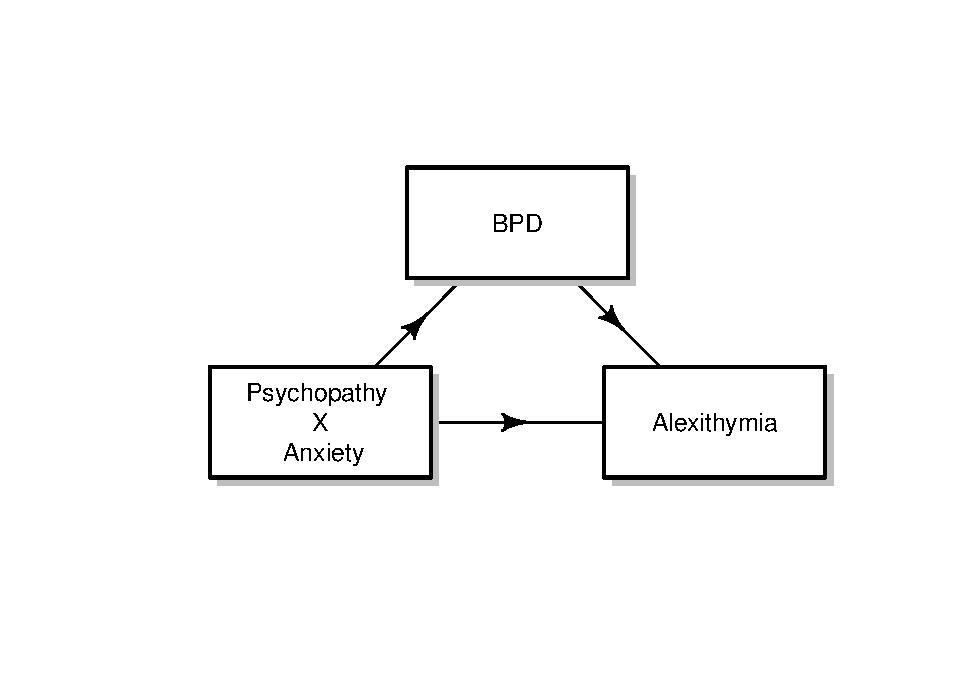
\includegraphics[width=1\linewidth]{d2m-Psychopathy_files/figure-latex/simple plot of mediation relationship-1} \caption{ }(\#fig:simple plot of mediation relationship)
\end{figure}

\hypertarget{methods}{%
\section{Methods}\label{methods}}

We report how we determined our sample size, all data exclusions (if any), all manipulations, and all measures in the study.

\hypertarget{participants}{%
\subsection{Participants}\label{participants}}

\hypertarget{measures}{%
\subsection{Measures}\label{measures}}

\hypertarget{procedure}{%
\subsection{Procedure}\label{procedure}}

\hypertarget{data-analysis}{%
\subsection{Data analysis}\label{data-analysis}}

We used R (Version 4.3.2; R Core Team, 2023) and the R-packages \emph{diagram} (Version 1.6.5; Soetaert, 2020), \emph{dplyr} (Version 1.1.4; Wickham, François, Henry, Müller, \& Vaughan, 2023), \emph{forcats} (Version 1.0.0; Wickham, 2023a), \emph{ggformula} (Version 0.12.0; Kaplan \& Pruim, 2023), \emph{ggplot2} (Version 3.4.4; Wickham, 2016), \emph{ggsci} (Version 3.0.0; Xiao, 2023), \emph{kableExtra} (Version 1.4.0; Zhu, 2024), \emph{lattice} (Version 0.21.9; Sarkar, 2008), \emph{lubridate} (Version 1.9.3; Grolemund \& Wickham, 2011), \emph{MASS} (Version 7.3.60; Venables \& Ripley, 2002), \emph{Matrix} (Version 1.6.1.1; Bates, Maechler, \& Jagan, 2023), \emph{mediation} (Imai, Keele, \& Tingley, 2010; Imai, Keele, Tingley, \& Yamamoto, 2011; Imai, Keele, \& Yamamoto, 2010; Imai \& Yamamoto, 2013; Version 4.5.0; Tingley, Yamamoto, Hirose, Keele, \& Imai, 2014), \emph{mosaic} (Version 1.9.0; Pruim, Kaplan, \& Horton, 2017; Pruim, Kaplan, \& Horton, 2023), \emph{mosaicData} (Version 0.20.4; Pruim et al., 2023), \emph{mvtnorm} (Version 1.2.4; Genz \& Bretz, 2009), \emph{papaja} (Version 0.1.2; Aust \& Barth, 2023), \emph{plot.matrix} (Version 1.6.2; Klinke, 2022), \emph{purrr} (Version 1.0.2; Wickham \& Henry, 2023), \emph{readr} (Version 2.1.4; Wickham, Hester, \& Bryan, 2023), \emph{readxl} (Version 1.4.3; Wickham \& Bryan, 2023), \emph{sandwich} (Zeileis, 2004, 2006; Version 3.1.0; Zeileis, Köll, \& Graham, 2020), \emph{shape} (Version 1.4.6; Soetaert, 2021), \emph{stargazer} (Version 5.2.3; Hlavac, 2022), \emph{stringr} (Version 1.5.1; Wickham, 2023b), \emph{tibble} (Version 3.2.1; Müller \& Wickham, 2023), \emph{tidyr} (Version 1.3.0; Wickham, Vaughan, \& Girlich, 2023), \emph{tidyverse} (Version 2.0.0; Wickham et al., 2019), and \emph{tinylabels} (Version 0.2.4; Barth, 2023) for all our analyses. Due to the nature of the project, it was determined most ethical to simply remove participants who were missing data for any of the required assessments. A total of 104 participants remained.

\hypertarget{results}{%
\section{Results}\label{results}}

Descriptive statistics for the assessments of interest can be seen in Table~\ref{tab:summary-table}.

\begin{table}[!htbp] \centering 
  \caption{} 
  \label{} 
\begin{tabular}{@{\extracolsep{5pt}}lccccc} 
\\[-1.8ex]\hline 
\hline \\[-1.8ex] 
Statistic & \multicolumn{1}{c}{N} & \multicolumn{1}{c}{Mean} & \multicolumn{1}{c}{St. Dev.} & \multicolumn{1}{c}{Min} & \multicolumn{1}{c}{Max} \\ 
\hline \\[-1.8ex] 
PAIBOR\_Total\_Score & 104 & 36.750 & 11.738 & 11 & 58 \\ 
PCLR\_Total\_Score\_Prorated & 104 & 23.476 & 8.070 & 4.400 & 37.000 \\ 
TAS\_Total\_Score & 104 & 49.702 & 13.852 & 20 & 82 \\ 
STAI\_Trait\_Anxiety & 104 & 45.558 & 11.213 & 23 & 72 \\ 
\hline \\[-1.8ex] 
\end{tabular} 
\end{table}

As seen in Figure~\ref{fig:PCLR-descriptives}, our distribution of PCL--R scores is left-skewed, with more participants falling on the higher end of the spectrum.



\begin{verbatim}
## Warning: Removed 2 rows containing missing values (`geom_bar()`).
\end{verbatim}

\begin{figure}
\centering
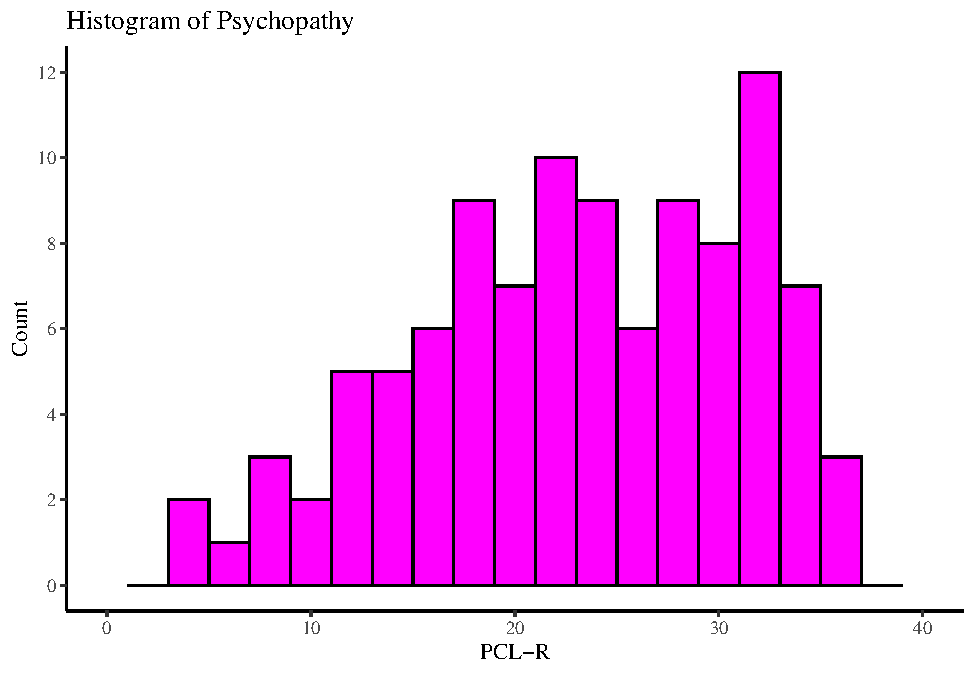
\includegraphics{d2m-Psychopathy_files/figure-latex/PCLR-descriptives-1.pdf}
\caption{\label{fig:PCLR-descriptives}Histogram of score distribution on the PCL--R.}
\end{figure}

\begin{verbatim}
## Warning: Removed 2 rows containing missing values (`geom_bar()`).
\end{verbatim}

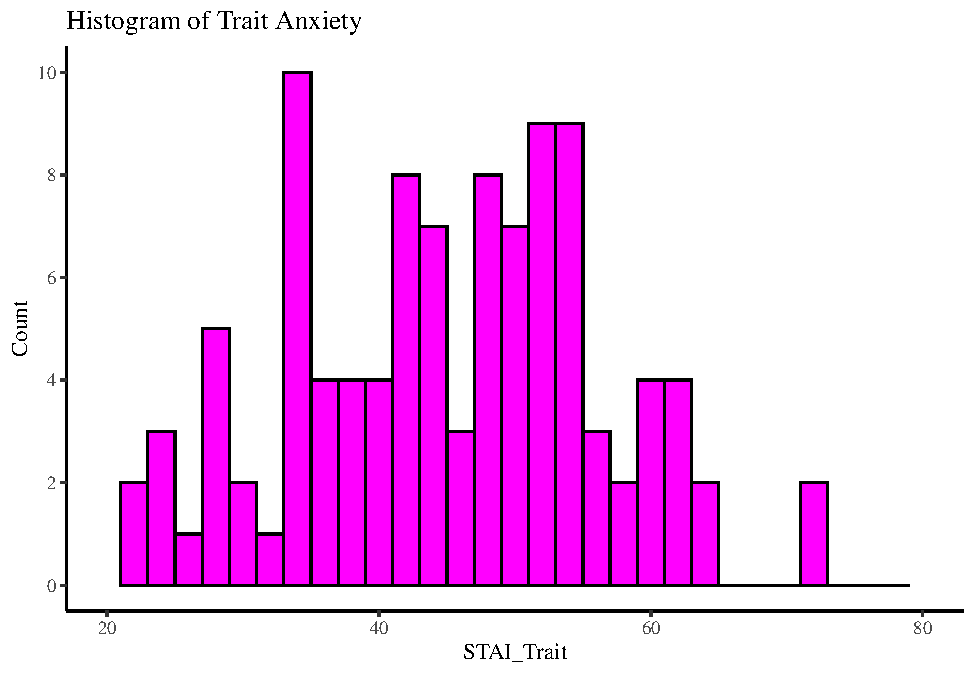
\includegraphics{d2m-Psychopathy_files/figure-latex/STAI-descriptives-1.pdf}

\begin{verbatim}
## Warning: Removed 1 rows containing missing values (`geom_bar()`).
\end{verbatim}

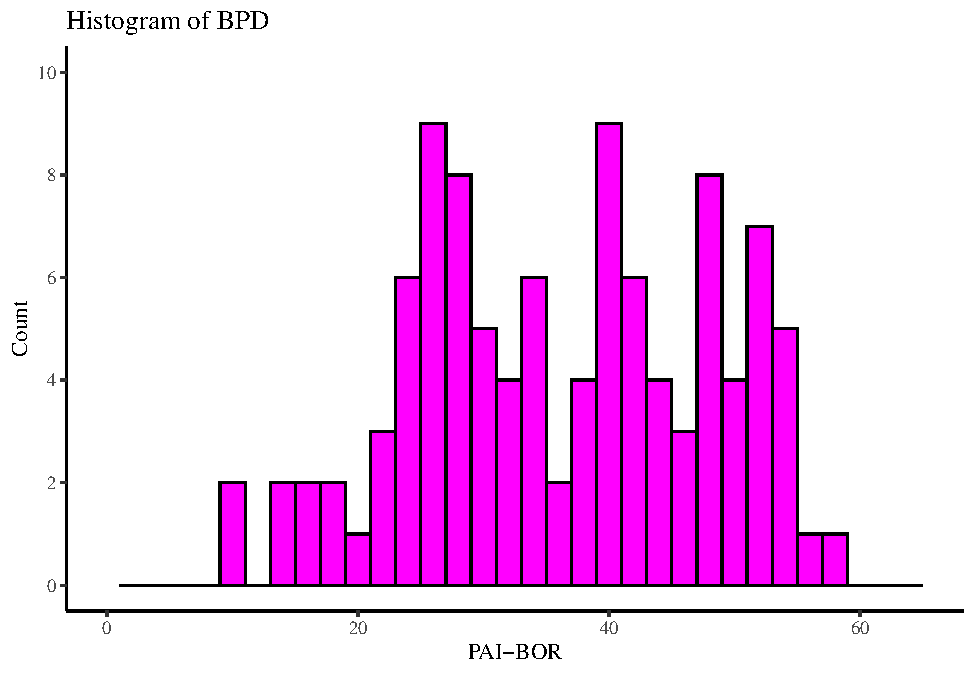
\includegraphics{d2m-Psychopathy_files/figure-latex/PAI-descriptives-1.pdf}

\begin{verbatim}
## Warning: Removed 1 rows containing non-finite values (`stat_bin()`).
\end{verbatim}

\begin{verbatim}
## Warning: Removed 2 rows containing missing values (`geom_bar()`).
\end{verbatim}

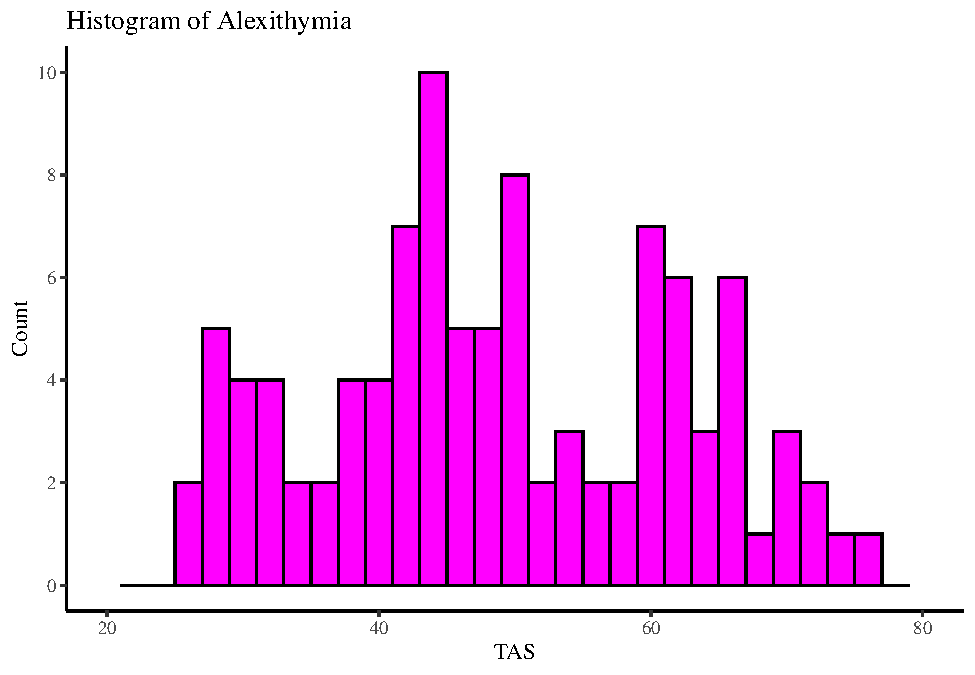
\includegraphics{d2m-Psychopathy_files/figure-latex/TAS-descriptives-1.pdf}

Figure~\ref{fig:c-path-scatterplot} shows a moderate correlation between PsychopathyXAnxiety and Alexithymia.



\begin{figure}
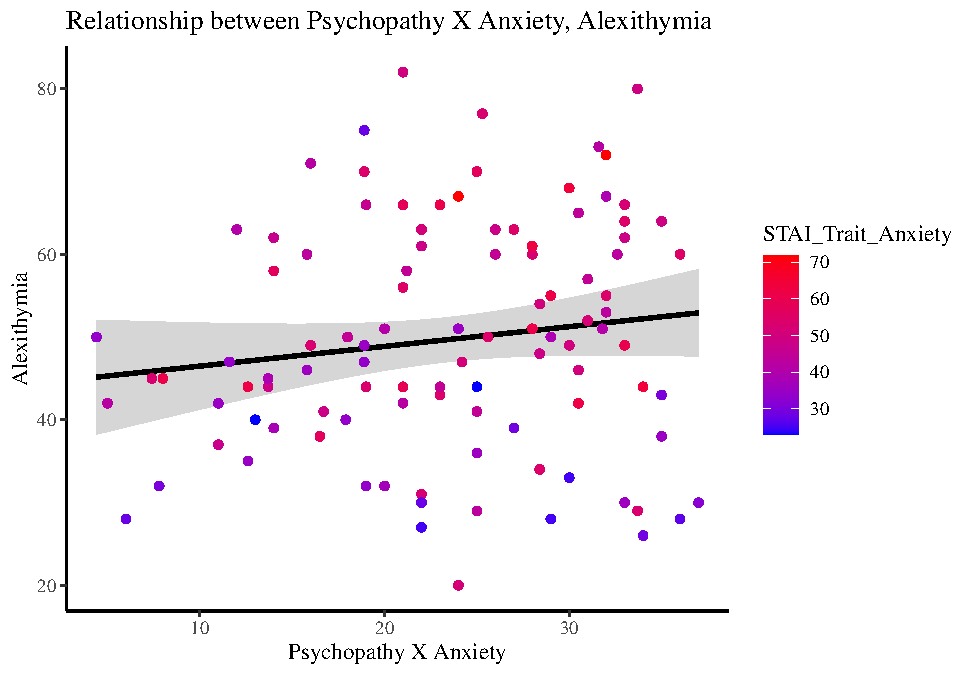
\includegraphics[width=1\linewidth]{d2m-Psychopathy_files/figure-latex/c-path-scatterplot-1} \caption{Scatterplot demonstrating relationship between the interactive term of psychopathy and trait anxiety with alexithymia in our sample of incarcerated women.}\label{fig:c-path-scatterplot}
\end{figure}

Figure~\ref{fig:a-path-scatterplot} shows a moderate to strong correlation between PsychopathyXAnxiety and BPD.



\begin{figure}
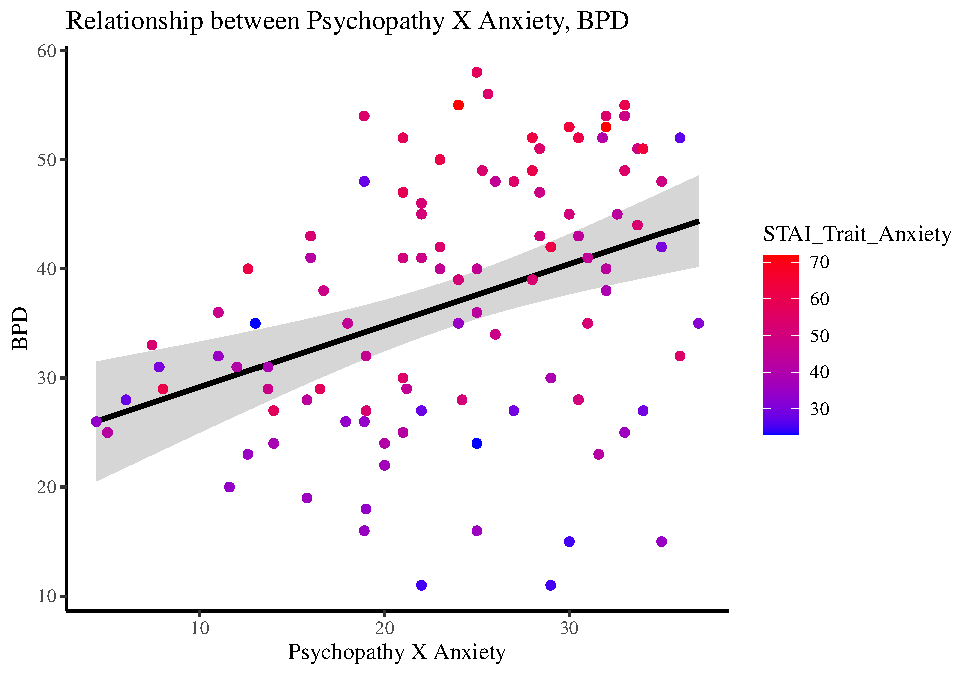
\includegraphics[width=1\linewidth]{d2m-Psychopathy_files/figure-latex/a-path-scatterplot-1} \caption{Scatterplot demonstrating relationship between the interactive term of psychopathy and trait anxiety with borderline personality disorder in our sample of incarcerated women.}\label{fig:a-path-scatterplot}
\end{figure}

All assessment scores (including the interactive term) were standardized. Mediation analyses with bootstrapping were conducted to test the primary hypothesis. Unlike other methods, bootstrapping is not limited by the assumption of normality. The interaction term of PCL--R Total Score and STAI Trait Anxiety was entered as the predictor, and PAI-BOR Total Score was entered as the mediating term. Total Score on the TAS was our outcome variable. A significant Average Causal Mediation Effect (ACME) would demonstrate support of our hypothesis. Summary tables (figure out how to include this info) show that the ACME is significant and the Average Direct Effect (ADE) disappears. This implies full causal mediation by BPD on the relationship between PsychopathyXAnxiety and Alexithymia.

In order to run a mediation analysis, one must ensure significant relationships exist between predictor and outcome, predictor and mediator, and mediator and outcome. Results for these preliminary analyses can be seen in some table somewhere.

\begin{table}[!htbp] \centering 
  \caption{Preliminary Regression Results} 
  \label{} 
\begin{tabular}{@{\extracolsep{1pt}}lccc} 
\\[-1.8ex]\hline 
\hline \\[-1.8ex] 
 & \multicolumn{3}{c}{\textit{Dependent variable:}} \\ 
\cline{2-4} 
\\[-1.8ex] & P-O Path & P-M Path & M-O Path \\ 
\\[-1.8ex] & (1) & (2) & (3)\\ 
\hline \\[-1.8ex] 
 PsychopathyXAnxiety & 0.373$^{***}$ & 0.660$^{***}$ &  \\ 
  & (0.092) & (0.074) &  \\ 
  & & & \\ 
 BPD &  &  & 0.471$^{***}$ \\ 
  &  &  & (0.087) \\ 
  & & & \\ 
 Constant & $-$0.000 & $-$0.000 & $-$0.000 \\ 
  & (0.091) & (0.074) & (0.087) \\ 
  & & & \\ 
\hline \\[-1.8ex] 
Observations & 104 & 104 & 104 \\ 
R$^{2}$ & 0.139 & 0.436 & 0.222 \\ 
Adjusted R$^{2}$ & 0.131 & 0.431 & 0.214 \\ 
Residual Std. Error (df = 102) & 0.932 & 0.755 & 0.887 \\ 
F Statistic (df = 1; 102) & 16.501$^{***}$ & 78.905$^{***}$ & 29.024$^{***}$ \\ 
\hline 
\hline \\[-1.8ex] 
\textit{Note:}  & \multicolumn{3}{r}{$^{*}$p$<$0.1; $^{**}$p$<$0.05; $^{***}$p$<$0.01} \\ 
\end{tabular} 
\end{table}

\begin{table}[!htbp] \centering 
  \caption{Simple Linear Regression Results} 
  \label{} 
\begin{tabular}{@{\extracolsep{1pt}}lcccc} 
\\[-1.8ex]\hline 
\hline \\[-1.8ex] 
 & \multicolumn{4}{c}{\textit{Dependent variable:}} \\ 
\cline{2-5} 
\\[-1.8ex] & TAS Total & Factor 1 & Factor 2 & Factor 3 \\ 
\\[-1.8ex] & (1) & (2) & (3) & (4)\\ 
\hline \\[-1.8ex] 
 PsychopathyXAnxiety & 0.373$^{***}$ & 0.418$^{***}$ & 0.291$^{***}$ & 0.197$^{**}$ \\ 
  & (0.092) & (0.090) & (0.095) & (0.097) \\ 
  & & & & \\ 
 Constant & $-$0.000 & $-$0.000 & $-$0.000 & 0.000 \\ 
  & (0.091) & (0.090) & (0.094) & (0.097) \\ 
  & & & & \\ 
\hline \\[-1.8ex] 
Observations & 104 & 104 & 104 & 104 \\ 
R$^{2}$ & 0.139 & 0.174 & 0.085 & 0.039 \\ 
Adjusted R$^{2}$ & 0.131 & 0.166 & 0.076 & 0.030 \\ 
Residual Std. Error (df = 102) & 0.932 & 0.913 & 0.961 & 0.985 \\ 
F Statistic (df = 1; 102) & 16.501$^{***}$ & 21.551$^{***}$ & 9.463$^{***}$ & 4.140$^{**}$ \\ 
\hline 
\hline \\[-1.8ex] 
\textit{Note:}  & \multicolumn{4}{r}{$^{*}$p$<$0.1; $^{**}$p$<$0.05; $^{***}$p$<$0.01} \\ 
\end{tabular} 
\end{table}

\begin{table}[!htbp] \centering 
  \caption{Multiple Linear Regression Results} 
  \label{} 
\begin{tabular}{@{\extracolsep{1pt}}lcccc} 
\\[-1.8ex]\hline 
\hline \\[-1.8ex] 
 & \multicolumn{4}{c}{\textit{Dependent variable:}} \\ 
\cline{2-5} 
\\[-1.8ex] & TAS Total & Factor 1 & Factor 2 & Factor 3 \\ 
\\[-1.8ex] & (1) & (2) & (3) & (4)\\ 
\hline \\[-1.8ex] 
 PsychopathyXAnxiety & 0.111 & 0.096 & 0.036 & 0.154 \\ 
  & (0.116) & (0.110) & (0.121) & (0.130) \\ 
  & & & & \\ 
 BPD & 0.398$^{***}$ & 0.487$^{***}$ & 0.386$^{***}$ & 0.066 \\ 
  & (0.116) & (0.110) & (0.121) & (0.130) \\ 
  & & & & \\ 
 Constant & $-$0.000 & $-$0.000 & $-$0.000 & 0.000 \\ 
  & (0.087) & (0.082) & (0.090) & (0.097) \\ 
  & & & & \\ 
\hline \\[-1.8ex] 
Observations & 104 & 104 & 104 & 104 \\ 
R$^{2}$ & 0.228 & 0.308 & 0.169 & 0.041 \\ 
Adjusted R$^{2}$ & 0.213 & 0.294 & 0.153 & 0.022 \\ 
Residual Std. Error (df = 101) & 0.887 & 0.840 & 0.921 & 0.989 \\ 
F Statistic (df = 2; 101) & 14.949$^{***}$ & 22.477$^{***}$ & 10.273$^{***}$ & 2.182 \\ 
\hline 
\hline \\[-1.8ex] 
\textit{Note:}  & \multicolumn{4}{r}{$^{*}$p$<$0.1; $^{**}$p$<$0.05; $^{***}$p$<$0.01} \\ 
\end{tabular} 
\end{table}

There is a significant relationship between predictor (psychopathy and anxiety interaction) and outcome (alexithymia). However, this effect goes away when adding BPD as a mediator. This suggests that the presence of BPD acts as a mechanism through which the predictor influences the outcome. The significant, full mediation effect we observed suggests that a portion of the total effect of the predictor on the outcome is explained by the mediator.

Three subfactors defined in the TAS are believed to compose alexithymia: difficulty identifying feelings (Factor 1), difficulty describing feelings (Factor 2), and externally-oriented thinking (Factor 3). As we collected subfactor scores for every participant, we decided to conduct an exploratory analysis to get a sense of what specific parts of emotional processing psychopathy and BPD may be impacting. We found that, replacing the total TAS score for Factor 1 and Factor 2, the significant mediation effect remained in tact. However, designating Factor 3 as an outcome left us with an insignificant model. The change in significant effect when replacing for specific factors of TAS suggests the mediation effect may depend on specific aspects or dimensions of alexithymia. I would like to suggest some possible interpretations for this below:

It is possible that BPD symptoms uniquely impact certain dimensions of the outcome variable. When considering what each of the three factors represent, it may be plausible that BPD would affect factors 1 and 2 -- addressing emotional comprehension and recognition -- and not 3, as BPD may be more closely associated with internalizing features. More research that addresses the role of BPD on externally-oriented thinking is required here to draw firmer conclusions.

It is without a doubt that the relationship between psychopathy, anxiety, BPD, and alexithymia is multifaceted and complex. Our results should be further interpreted with caution and a unique sample such as this one may lead to skewed distributions.

Additional factors and moderators warrant further exploration. Other relevant comorbidities -- such as PTSD -- may influence the heterogeneous mediation pathway seen here in a way that could explain the nuanced relationships further. Further, it would certainly be worthwhile to break down BPD further to understand what specific mechanisms of this disorder might be at play in this relationship. We did not have sufficient data to conduct a factor analysis, but it may be useful as the personality disorder can be diagnosed in 256 unique ways, according to the DSM-V.

The heterogeneity of this mediation effect is certainly cause for future research. This information can guide the development of targeted interventions or strategies based on specific factors that are most influenced by the mediation process. This changes in significance emphasize the need for careful and nuanced interpretation, taking into account the specific characteristics and dynamics at play for each factor within the composite variables.

\hypertarget{discussion}{%
\section{Discussion}\label{discussion}}

\newpage

\hypertarget{references}{%
\section{References}\label{references}}

\hypertarget{refs}{}
\begin{CSLReferences}{1}{0}
\leavevmode\vadjust pre{\hypertarget{ref-R-papaja}{}}%
Aust, F., \& Barth, M. (2023). \emph{{papaja}: {Prepare} reproducible {APA} journal articles with {R Markdown}}. Retrieved from \url{https://github.com/crsh/papaja}

\leavevmode\vadjust pre{\hypertarget{ref-R-tinylabels}{}}%
Barth, M. (2023). \emph{{tinylabels}: Lightweight variable labels}. Retrieved from \url{https://cran.r-project.org/package=tinylabels}

\leavevmode\vadjust pre{\hypertarget{ref-R-Matrix}{}}%
Bates, D., Maechler, M., \& Jagan, M. (2023). \emph{Matrix: Sparse and dense matrix classes and methods}. Retrieved from \url{https://CRAN.R-project.org/package=Matrix}

\leavevmode\vadjust pre{\hypertarget{ref-R-mvtnorm}{}}%
Genz, A., \& Bretz, F. (2009). \emph{Computation of multivariate normal and t probabilities}. Heidelberg: Springer-Verlag.

\leavevmode\vadjust pre{\hypertarget{ref-R-lubridate}{}}%
Grolemund, G., \& Wickham, H. (2011). Dates and times made easy with {lubridate}. \emph{Journal of Statistical Software}, \emph{40}(3), 1--25. Retrieved from \url{https://www.jstatsoft.org/v40/i03/}

\leavevmode\vadjust pre{\hypertarget{ref-R-stargazer}{}}%
Hlavac, M. (2022). \emph{Stargazer: Well-formatted regression and summary statistics tables}. Bratislava, Slovakia: Social Policy Institute. Retrieved from \url{https://CRAN.R-project.org/package=stargazer}

\leavevmode\vadjust pre{\hypertarget{ref-R-mediation_c}{}}%
Imai, K., Keele, L., \& Tingley, D. (2010). A general approach to causal mediation analysis. \emph{Psychological Methods}, \emph{15}(4), 309--334. Retrieved from \url{http://imai.princeton.edu/research/BaronKenny.html}

\leavevmode\vadjust pre{\hypertarget{ref-R-mediation_d}{}}%
Imai, K., Keele, L., Tingley, D., \& Yamamoto, T. (2011). Unpacking the black box of causality: Learning about causal mechanisms from experimental and observational studies. \emph{American Political Science Review}, \emph{105}(4), 765--789. Retrieved from \url{http://imai.princeton.edu/research/mediationP.html}

\leavevmode\vadjust pre{\hypertarget{ref-R-mediation_b}{}}%
Imai, K., Keele, L., \& Yamamoto, T. (2010). Identification, inference, and sensitivity analysis for causal mediation effects. \emph{Statistical Science}, \emph{25}(1), 51--71. Retrieved from \url{http://imai.princeton.edu/research/mediation.html}

\leavevmode\vadjust pre{\hypertarget{ref-R-mediation_e}{}}%
Imai, K., \& Yamamoto, T. (2013). Identification and sensitivity analysis for multiple causal mechanisms: Revisiting evidence from framing experiments. \emph{Political Analysis}, \emph{21}(2), 141--171. Retrieved from \url{http://imai.princeton.edu/research/medsens.html}

\leavevmode\vadjust pre{\hypertarget{ref-R-ggformula}{}}%
Kaplan, D., \& Pruim, R. (2023). \emph{Ggformula: Formula interface to the grammar of graphics}. Retrieved from \url{https://CRAN.R-project.org/package=ggformula}

\leavevmode\vadjust pre{\hypertarget{ref-R-plot.matrix}{}}%
Klinke, S. (2022). \emph{Plot.matrix: Visualizes a matrix as heatmap}. Retrieved from \url{https://CRAN.R-project.org/package=plot.matrix}

\leavevmode\vadjust pre{\hypertarget{ref-R-tibble}{}}%
Müller, K., \& Wickham, H. (2023). \emph{Tibble: Simple data frames}. Retrieved from \url{https://CRAN.R-project.org/package=tibble}

\leavevmode\vadjust pre{\hypertarget{ref-R-mosaic}{}}%
Pruim, R., Kaplan, D. T., \& Horton, N. J. (2017). The mosaic package: Helping students to 'think with data' using r. \emph{The R Journal}, \emph{9}(1), 77--102. Retrieved from \url{https://journal.r-project.org/archive/2017/RJ-2017-024/index.html}

\leavevmode\vadjust pre{\hypertarget{ref-R-mosaicData}{}}%
Pruim, R., Kaplan, D., \& Horton, N. (2023). \emph{mosaicData: Project MOSAIC data sets}. Retrieved from \url{https://CRAN.R-project.org/package=mosaicData}

\leavevmode\vadjust pre{\hypertarget{ref-R-base}{}}%
R Core Team. (2023). \emph{R: A language and environment for statistical computing}. Vienna, Austria: R Foundation for Statistical Computing. Retrieved from \url{https://www.R-project.org/}

\leavevmode\vadjust pre{\hypertarget{ref-R-lattice}{}}%
Sarkar, D. (2008). \emph{Lattice: Multivariate data visualization with r}. New York: Springer. Retrieved from \url{http://lmdvr.r-forge.r-project.org}

\leavevmode\vadjust pre{\hypertarget{ref-R-diagram}{}}%
Soetaert, K. (2020). \emph{Diagram: Functions for visualising simple graphs (networks), plotting flow diagrams}. Retrieved from \url{https://CRAN.R-project.org/package=diagram}

\leavevmode\vadjust pre{\hypertarget{ref-R-shape}{}}%
Soetaert, K. (2021). \emph{Shape: Functions for plotting graphical shapes, colors}. Retrieved from \url{https://CRAN.R-project.org/package=shape}

\leavevmode\vadjust pre{\hypertarget{ref-R-mediation_a}{}}%
Tingley, D., Yamamoto, T., Hirose, K., Keele, L., \& Imai, K. (2014). {mediation}: {R} package for causal mediation analysis. \emph{Journal of Statistical Software}, \emph{59}(5), 1--38. Retrieved from \url{http://www.jstatsoft.org/v59/i05/}

\leavevmode\vadjust pre{\hypertarget{ref-R-MASS}{}}%
Venables, W. N., \& Ripley, B. D. (2002). \emph{Modern applied statistics with s} (Fourth). New York: Springer. Retrieved from \url{https://www.stats.ox.ac.uk/pub/MASS4/}

\leavevmode\vadjust pre{\hypertarget{ref-R-ggplot2}{}}%
Wickham, H. (2016). \emph{ggplot2: Elegant graphics for data analysis}. Springer-Verlag New York. Retrieved from \url{https://ggplot2.tidyverse.org}

\leavevmode\vadjust pre{\hypertarget{ref-R-forcats}{}}%
Wickham, H. (2023a). \emph{Forcats: Tools for working with categorical variables (factors)}. Retrieved from \url{https://CRAN.R-project.org/package=forcats}

\leavevmode\vadjust pre{\hypertarget{ref-R-stringr}{}}%
Wickham, H. (2023b). \emph{Stringr: Simple, consistent wrappers for common string operations}. Retrieved from \url{https://CRAN.R-project.org/package=stringr}

\leavevmode\vadjust pre{\hypertarget{ref-R-tidyverse}{}}%
Wickham, H., Averick, M., Bryan, J., Chang, W., McGowan, L. D., François, R., \ldots{} Yutani, H. (2019). Welcome to the {tidyverse}. \emph{Journal of Open Source Software}, \emph{4}(43), 1686. \url{https://doi.org/10.21105/joss.01686}

\leavevmode\vadjust pre{\hypertarget{ref-R-readxl}{}}%
Wickham, H., \& Bryan, J. (2023). \emph{Readxl: Read excel files}. Retrieved from \url{https://CRAN.R-project.org/package=readxl}

\leavevmode\vadjust pre{\hypertarget{ref-R-dplyr}{}}%
Wickham, H., François, R., Henry, L., Müller, K., \& Vaughan, D. (2023). \emph{Dplyr: A grammar of data manipulation}. Retrieved from \url{https://CRAN.R-project.org/package=dplyr}

\leavevmode\vadjust pre{\hypertarget{ref-R-purrr}{}}%
Wickham, H., \& Henry, L. (2023). \emph{Purrr: Functional programming tools}. Retrieved from \url{https://CRAN.R-project.org/package=purrr}

\leavevmode\vadjust pre{\hypertarget{ref-R-readr}{}}%
Wickham, H., Hester, J., \& Bryan, J. (2023). \emph{Readr: Read rectangular text data}. Retrieved from \url{https://CRAN.R-project.org/package=readr}

\leavevmode\vadjust pre{\hypertarget{ref-R-tidyr}{}}%
Wickham, H., Vaughan, D., \& Girlich, M. (2023). \emph{Tidyr: Tidy messy data}. Retrieved from \url{https://CRAN.R-project.org/package=tidyr}

\leavevmode\vadjust pre{\hypertarget{ref-R-ggsci}{}}%
Xiao, N. (2023). \emph{Ggsci: Scientific journal and sci-fi themed color palettes for 'ggplot2'}. Retrieved from \url{https://CRAN.R-project.org/package=ggsci}

\leavevmode\vadjust pre{\hypertarget{ref-R-sandwich_b}{}}%
Zeileis, A. (2004). Econometric computing with {HC} and {HAC} covariance matrix estimators. \emph{Journal of Statistical Software}, \emph{11}(10), 1--17. \url{https://doi.org/10.18637/jss.v011.i10}

\leavevmode\vadjust pre{\hypertarget{ref-R-sandwich_c}{}}%
Zeileis, A. (2006). Object-oriented computation of sandwich estimators. \emph{Journal of Statistical Software}, \emph{16}(9), 1--16. \url{https://doi.org/10.18637/jss.v016.i09}

\leavevmode\vadjust pre{\hypertarget{ref-R-sandwich_a}{}}%
Zeileis, A., Köll, S., \& Graham, N. (2020). Various versatile variances: An object-oriented implementation of clustered covariances in {R}. \emph{Journal of Statistical Software}, \emph{95}(1), 1--36. \url{https://doi.org/10.18637/jss.v095.i01}

\leavevmode\vadjust pre{\hypertarget{ref-R-kableExtra}{}}%
Zhu, H. (2024). \emph{kableExtra: Construct complex table with 'kable' and pipe syntax}. Retrieved from \url{https://CRAN.R-project.org/package=kableExtra}

\end{CSLReferences}


\end{document}
